\chapter{The Booster Neutrino Beam}\label{ch:beam}
The MicroBooNE detector is stationed at FNAL where it receives neutrinos from both the Booster Neutrino Beam (BNB) and Neutrinos from the Main Injector (NuMI) beams. MicroBooNE is on-axis for the BNB and off-axis by 135 mrad for NuMI. The BNB is a very pure $\nu_{\mu}$ beam, with only 0.6\% contamination from $\nu_{e}s$. The energy also peaks around 700 MeV which is desired based on the probability of oscillation equation which depends on the the value of $L/E$, where $L$ is the distance of the detector from the neutrino beam and $E$ is the energy of the neutrino beam. $L/E$ was chosen to increase the probability of seeing neutrino oscillations in the MiniBooNE Low Energy Excess (LEE) range based on the probability of oscillation equation is $ P_{\nu_{\mu}\rightarrow \nu_{e}}\left(L,E\right) = \sin^2 2\theta \sin^2 \left(1.27\Delta m^2 \frac{L}{E_{\nu}}\right)$. The Short Baseline Neutrino (SBN) Program will further study non-standard neutrino oscillations and is composed of 3 LArTPCs including the MicroBooNE experiement \cite{SBN}. MicroBooNE's second goal is to gain a cross section measurement on $\nu-Ar$. MicroBooNE's neutrino cross-section program will be the first $\nu-Ar$ cross-section in the 1 GeV energy range and one of only a few cross-section measurements of $\nu-Ar$ in the world. This has significance in part because of the large scale LArTPCs slated for construction over the next decade \cite{dune} \cite{SBN}. 


\begin{figure}[htp!]
\centering
	\begin{subfigure}[b]{.4\textwidth}
	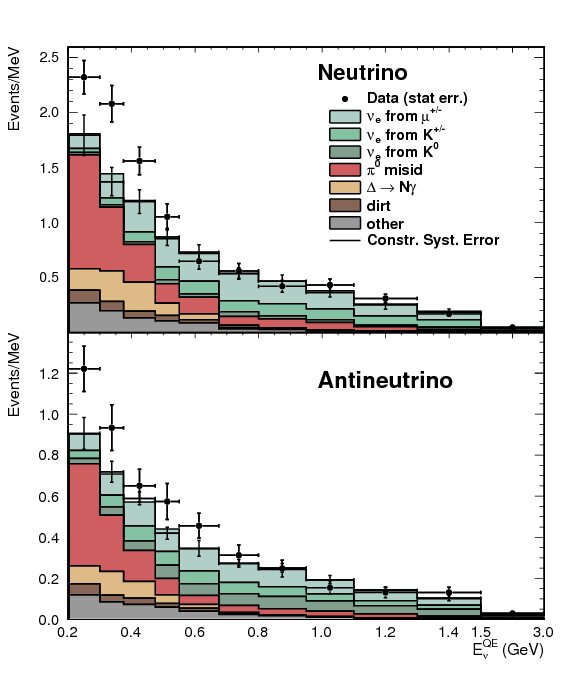
\includegraphics[width=\textwidth]{figs/lee.png}
	\caption{Low Energy excess seen in MiniBooNE}
	\label{fig:lee}
	\end{subfigure}
	\quad
	\begin{subfigure}[b]{.4\textwidth}
	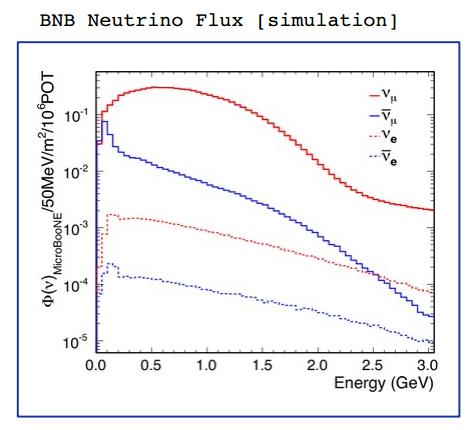
\includegraphics[width=\textwidth]{figs/bnbflux.png}
	\caption{Energy spectrum of the Booster Neutrino Beam at Fermi National Laboratories}
	\label{fig:bnbflux}
	\end{subfigure}
	\quad
\label{fig:figures}
\caption{\ref{fig:bnbflux} Flux of BNB at FNAL.}
\end{figure}
